\documentclass[11pt]{amsart}
\usepackage[margin=1.15in]{geometry}
\usepackage{amsmath,amssymb}
\usepackage{booktabs}
\usepackage{graphicx}
\usepackage[hidelinks]{hyperref}
\usepackage{url}

\newtheorem{theorem}{Theorem}[section]
\newtheorem{lemma}[theorem]{Lemma}
\newtheorem{proposition}[theorem]{Proposition}
\newtheorem{remark}[theorem]{Remark}
\newcommand{\Kq}[3]{K_{#1}(#2,#3)}
\newcommand{\Zq}{\mathbb{Z}_q}

% AUTO-GENERATED by scripts/paper_tables.py -- do not edit by hand.
\newcommand{\ubtable}{%
\begin{tabular}{lcccccl}
\toprule
cell & previous bounds & new UB & $\Delta$ & $\Delta\%$ & key & previous UB via \\
\midrule
$\Kq{5}{11}{5}$ & 103--625 & \textbf{602} & $-23$ & $3.7\%$ & \texttt{d} & Bhandari--Durairajan 1996 \\
$\Kq{6}{7}{3}$ & 70--246 & \textbf{227} & $-19$ & $7.7\%$ & \texttt{e} & $K_q(n{+}1,R)\le q\,K_q(n,R)$ \\
$\Kq{6}{8}{3}$ & 246--1080 & \textbf{1005} & $-75$ & $6.9\%$ & \texttt{f} & direct sum \\
$\Kq{6}{8}{4}$ & 46--216 & \textbf{166} & $-50$ & $23.1\%$ & \texttt{e} & $K_q(n{+}1,R)\le q\,K_q(n,R)$ \\
$\Kq{6}{9}{4}$ & 136--738 & \textbf{660} & $-78$ & $10.6\%$ & \texttt{f} & direct sum \\
$\Kq{6}{9}{5}$ & 32--144 & \textbf{119} & $-25$ & $17.4\%$ & \texttt{j} & alphabet product rule \\
$\Kq{6}{10}{4}$ & \textbf{441}--2952 & \textbf{2781}$^{\downarrow}$ & $-171$ & $5.8\%$ & \texttt{f} & direct sum \\
$\Kq{6}{10}{5}$ & 83--615 & \textbf{486}$^{\downarrow}$ & $-129$ & $21.0\%$ & \texttt{f} & direct sum \\
$\Kq{7}{8}{4}$ & 76--343 & \textbf{316} & $-27$ & $7.9\%$ & \texttt{c} & monotonicity $K_q(n{+}1,R{+}1)\le K_q(n,R)$ \\
$\Kq{7}{9}{4}$ & 264--1843 & \textbf{1475}$^{\downarrow}$ & $-368$ & $20.0\%$ & \texttt{f} & direct sum \\
$\Kq{8}{6}{4}$ & 15--20 & \textbf{19}$^{\downarrow}$ & $-1$ & $5.0\%$ & \texttt{n} & K\'eri--\"Osterg\aa rd 2005 \\
$\Kq{8}{8}{4}$ & 118--512 & \textbf{505} & $-7$ & $1.4\%$ & \texttt{c} & monotonicity $K_q(n{+}1,R{+}1)\le K_q(n,R)$ \\
$\Kq{8}{8}{5}$ & 29--90 & \textbf{85}$^{\downarrow}$ & $-5$ & $5.6\%$ & \texttt{z} & K\'eri 2009 \\
$\Kq{8}{10}{6}$ & 58--342 & \textbf{341}$^{\downarrow}$ & $-1$ & $0.3\%$ & \texttt{n} & K\'eri--\"Osterg\aa rd 2005 \\
$\Kq{12}{6}{4}$ & 30--41 & \textbf{39}$^{\downarrow}$ & $-2$ & $4.9\%$ & \texttt{q} & Rivas Soriano 2005--2008 \\
$\Kq{13}{6}{4}$ & 35--46 & \textbf{45}$^{\downarrow}$ & $-1$ & $2.2\%$ & \texttt{q} & Rivas Soriano 2005--2008 \\
$\Kq{14}{6}{4}$ & 40--52 & \textbf{50}$^{\downarrow}$ & $-2$ & $3.8\%$ & \texttt{q} & Rivas Soriano 2005--2008 \\
$\Kq{15}{6}{4}$ & 46--59 & \textbf{57}$^{\downarrow}$ & $-2$ & $3.4\%$ & \texttt{c} & monotonicity $K_q(n{+}1,R{+}1)\le K_q(n,R)$ \\
\bottomrule
\end{tabular}}
\newcommand{\lbtable}{%
\begin{tabular}{lccccc}
\toprule
cell & sphere bound & previous LB (key) & new LB & SDP value$^{1/3}$ & known UB \\
\midrule
$\Kq{6}{9}{3}$ & 881 & 921 (\texttt{y}) & \textbf{924} & $923.9804$ & 4752 \\
$\Kq{6}{10}{4}$ & 411 & 417 (\texttt{s}) & \textbf{441} & $440.2854$ & 2952 \\
$\Kq{7}{8}{3}$ & 439 & 457 (\texttt{y}) & \textbf{471} & $470.3230$ & 2337 \\
$\Kq{8}{8}{3}$ & 813 & 829 (\texttt{y}) & \textbf{855} & $854.5627$ & 4096 \\
$\Kq{8}{9}{4}$ & 403 & 409 (\texttt{s}) & \textbf{428} & $427.4131$ & 2944 \\
$\Kq{9}{9}{4}$ & 690 & 703 (\texttt{s}) & \textbf{718} & $717.8794$ & 5103 \\
$\Kq{10}{9}{4}$ & 1123 & 1130 (\texttt{s}) & \textbf{1145} & $1144.1984$ & 8500 \\
\bottomrule
\end{tabular}}


\title[New bounds on covering codes for $5\le q\le 21$]{New upper and lower
bounds on covering codes $K_q(n,R)$\\ for alphabets of size $5\le q\le 21$}
\author{Mark Marosi}
\thanks{Department of Measurement and Information Systems, Budapest
University of Technology and Economics (BME), Budapest, Hungary.
Email: \texttt{marosi@mit.bme.hu}.}
\thanks{This work was carried out in collaboration with the AI system
Claude (Anthropic); the division of contributions is stated at the end of
the paper.}
\subjclass[2020]{94B75 (primary), 05B40, 90C22, 90C59}
\keywords{Covering codes, football pool problem, semidefinite programming,
local search, large-neighbourhood search, GPU computing}
\date{August 2026}

\begin{document}

\begin{abstract}
Let $K_q(n,R)$ denote the minimum cardinality of a $q$-ary code of length
$n$ with covering radius $R$. We improve the known bounds on $K_q(n,R)$ in
$83$ cases ($82$ distinct cells). On the upper-bound side we give $25$
improved bounds for $5\le q\le 15$ --- twenty-four found by search and one
propagated by monotonicity --- using two complementary methods: an
engineered
focused local search seeded with structural constructions, and a
large-neighbourhood search driven by exact full-space coverage transforms
that evaluates every candidate codeword position simultaneously. These are,
to our knowledge, the first improvements to any upper bound on $K_q(n,R)$
with $q\ge 5$ since the 2011 revision of K\'eri's tables; several bounds
decrease by more than $20\%$, e.g.\ $\Kq{6}{8}{4}\le 166$ (previously
$216$) and $\Kq{8}{10}{5}\le 1883$ (previously $2461$). On the lower-bound
side we give $58$ improved bounds for $6\le q\le 21$, obtained from the
semidefinite programming hierarchy of Gijswijt and Polak, whose published
results cover $q\le 5$, by combining an exact-arithmetic reimplementation
of the reduced program with a multiprecision solution pipeline. Every new
lower bound is certified by a rational dual solution validated by a
standalone exact-arithmetic checker; no floating-point computation is part
of the trusted base. The same pipeline also gives strong numerical
evidence of limits: on a dozen further cells the certified value of the
relaxation, which the solver reports as optimal to within its working
precision, lies below the best known bound, indicating that no improvement
is available there at this level of the hierarchy. One cell is improved
from both sides:
$441\le \Kq{6}{10}{4}\le 2751$, previously $417$--$2952$. All codes and
certificates are provided in machine-readable form together with standalone
verifiers.
\end{abstract}

\maketitle

\section{Introduction}

Let $\Zq^n$ denote the Hamming space of $q$-ary words of length $n$. A code
$C\subseteq \Zq^n$ has \emph{covering radius} $R$ if every word of $\Zq^n$
is within Hamming distance $R$ of some codeword, and
\[
K_q(n,R) \;=\; \min\{\,|C| : C\subseteq \Zq^n \text{ has covering radius}
\le R\,\}.
\]
The function $K_q(n,R)$ is a central quantity of covering-code
theory~\cite{CHLL}; the binary case $K_2(n,1)$ includes the domination
number of the hypercube, and $K_3(n,1)$ is the classical football pool
problem.

Upper bounds on $K_q(n,R)$ are established by explicit constructions and
lower bounds by combinatorial or convex-relaxation arguments; the state of
the art is recorded in the tables of K\'eri~\cite{Keri}, which subsume and
extend those of~\cite{CHLL} and were last revised in November 2011. Recent
work has concentrated on lower bounds for small alphabets: Wu and
Chen~\cite{WuChen} improved binary lower bounds via congruence arguments,
and Gijswijt and Polak~\cite{GijswijtPolak} obtained many new lower bounds
for $q\le 5$ from a semidefinite programming hierarchy; a complementary
line of work formalizes covering-code bounds in a proof
assistant~\cite{Florath}. The lower-bound results of~\cite{GijswijtPolak}
include improvements at $q=5$; for $q\ge 6$ we are not aware of any
published improvement on either side since 2011, nor of any on the
upper-bound side for $q\ge 5$; a
systematic search of the literature (arXiv, DBLP, OpenAlex, Lobstein's
covering-radius bibliography~\cite{Lobstein}, and the publication lists of
the authors active in the area, performed in August 2026) found none.

This paper improves both sides of the tables in that range. Our
contributions are the following.
\begin{enumerate}
\item \emph{New upper bounds.} Twenty-five improved upper bounds for
$5\le q\le 15$ (Table~\ref{tab:ub}), each an explicit code ---
twenty-four found by direct search and one propagated from another by
monotonicity. The searches use two complementary methods: an engineered
focused local search seeded with structural constructions
(Section~\ref{sec:method}), effective for $q^n\lesssim 10^8$, and a
large-neighbourhood search driven by exact full-space coverage transforms
(Section~\ref{sec:gpu}), which evaluates \emph{every} candidate placement
simultaneously and extends the searchable range to $q^n=10^{10}$.
\item \emph{New lower bounds.} Fifty-eight improved lower bounds for
$6\le q\le 21$ (Table~\ref{tab:lb}), obtained by solving the
symmetry-reduced semidefinite relaxation of Gijswijt and
Polak~\cite{GijswijtPolak} in multiprecision arithmetic and rounding each
numerical dual solution to an exact rational certificate
(Section~\ref{sec:lb}). The certificates are self-contained: a standalone
exact-arithmetic checker re-derives the program and validates each one, so
no floating-point computation is part of the trusted base.
\item \emph{Evidence of limits.} On a dozen further cells the same
pipeline produces a certified value strictly below the tabulated bound,
with the solver reporting optimality of the relaxation to within its
working precision (Section~\ref{sec:lb:limits}); this is strong numerical
evidence --- though, as we are careful to state, not an exact
certificate --- that those cells resist improvement at this level of the
hierarchy.
\item \emph{Verification.} Every claimed bound is verified independently of
the software that produced it (Section~\ref{sec:verify}); all codes,
certificates, and both standalone verifiers are published in
machine-readable form.
\end{enumerate}

Two structural observations locate the improvements. On the upper-bound
side, K\'eri's source annotations show that for moderate $q$ and $R\ge 3$
most tabulated bounds are inherited from the general constructions of
Section~\ref{sec:prelim} rather than from search in the cell itself. Such
bounds decrease the furthest under direct search (by up to $23\%$); bounds
previously obtained by dedicated search in the
2000s~\cite{KeriOstergard2005} also decrease, by $2$--$12\%$. On the lower-bound side, the size of the symmetry-reduced
Gijswijt--Polak semidefinite program depends only on $n$ and not on $q$, so
the restriction of the published results to $q\le 5$ is consistent with
numerical precision, rather than model size, being the binding
constraint; solving the same relaxation in
multiprecision arithmetic and certifying the results exactly yields
improvements throughout $6\le q\le 21$, concentrated on the cells whose
incumbent lower bounds are close to the sphere-covering bound.

The paper is organized as follows. Section~\ref{sec:prelim} fixes notation.
Section~\ref{sec:results} states the results.
Sections~\ref{sec:method} and~\ref{sec:gpu} describe the two upper-bound
search methods, Section~\ref{sec:lb} the lower-bound pipeline, and
Section~\ref{sec:verify} the verification protocol applied to every claimed
bound. Implementation details and the controlled measurements supporting
the engineering claims are collected in Appendix~\ref{app:impl}; the
largest relative improvement, the code proving $\Kq{6}{8}{4}\le 166$, is
printed in Appendix~\ref{app:code}.

\section{Preliminaries}\label{sec:prelim}

Throughout, $q\ge 2$ and $\Zq=\{0,\dots,q-1\}$; $d(x,y)$ denotes Hamming
distance on $\Zq^n$, $B_R(x)=\{y: d(x,y)\le R\}$ the Hamming ball, and
$|B_R|=\sum_{i\le R}\binom{n}{i}(q-1)^i$ its volume. Counting yields the
\emph{sphere-covering bound}
$K_q(n,R)\ \ge\ \lceil q^n/|B_R|\rceil$.

The classical constructions that propagate upper bounds through the tables
are the \emph{direct sum}
\begin{equation}\label{eq:directsum}
K_q(n_1+n_2,\,R_1+R_2)\;\le\;K_q(n_1,R_1)\cdot K_q(n_2,R_2),
\end{equation}
the length rule $K_q(n+1,R)\le q\,K_q(n,R)$, the monotonicity
$K_q(n+1,R+1)\le K_q(n,R)$, and product rules over alphabet factorizations;
see~\cite{CHLL,Keri} for these and for the source annotations (``keys'')
used in the tables below. For a code $C$ of size $M$ we write
$\mathrm{cnt}(w)=\#\{c\in C: d(w,c)\le R\}$ for the coverage multiplicity
of a word $w$; $C$ is a cover if and only if $\mathrm{cnt}>0$ everywhere.

\section{The new bounds}\label{sec:results}

Tables~\ref{tab:ub} and~\ref{tab:lb} list the new bounds;
Figure~\ref{fig:summary} summarizes both sides. We note the following.

\begin{enumerate}
\item The cell $\Kq{6}{10}{4}$ is improved from both sides, from
$417$--$2952$ to $441$--$2751$.
\item None of the upper-bound searches is known to be exhausted. The
highest-redundancy cells (e.g.\ $\Kq{7}{9}{4}$, $\Kq{6}{10}{4}$,
$\Kq{8}{10}{5}$) improved at every escalation of the computational budget
before reaching their final values;
the bounds marked ${}^{\downarrow}$ in Table~\ref{tab:ub} are the values at
the time of writing, not limits of the method.
\item The lower-bound improvements are concentrated where the incumbents
are weakest relative to the sphere-covering bound. All $58$ improved cells
carry K\'eri keys \texttt{y}, \texttt{x}, \texttt{s} or \texttt{a} (bounds
within a few percent of sphere-covering); the entire family
$(n,R)=(8,2)$, $6\le q\le 21$, is improved at once, the increments growing
from $+91$ at $q=6$ to
$+14436$ at $q=21$, and the largest single increment is
$\Kq{10}{10}{2}\ge 2699348$, previously $2676660$. No cell whose incumbent
is due to Haas, Halupczok and Schlage-Puchta~\cite{HHSP2009}
(key \texttt{m}) is improved;
Section~\ref{sec:lb:limits} quantifies this limitation.
\item One further upper bound is obtained by propagating a new bound
through the rules of Section~\ref{sec:prelim} rather than by direct
search: the new $\Kq{7}{8}{4}\le 316$ gives $\Kq{7}{9}{5}\le 316$
(previously $323$) by monotonicity, realized as an explicit code by
appending a fixed coordinate; the code was verified like every other. We
checked that the closure of all new bounds under the propagation rules
yields no further improvement beyond the observation of
Remark~\ref{rem:keri17}.
\end{enumerate}

\begin{table}[t]
\centering
\small
\ubtable
\caption{New upper bounds. ``Previous bounds'' are the lower--upper pairs
of K\'eri's tables~\cite{Keri}; a bold lower bound is from
Table~\ref{tab:lb} of this paper. ``Sphere'' is the sphere-covering bound
$\lceil q^n/|B_R|\rceil$. ``Key'' is the source annotation of the
previous upper bound in~\cite{Keri}: \ubkeylegend. ``Via'' names the
producing method: L $=$ the local search of Section~\ref{sec:method},
T $=$ the transform engine of Section~\ref{sec:gpu}, M $=$ monotonicity
propagation of another new bound. Percentages are rounded to one decimal.
A ${}^{\downarrow}$ marks bounds whose descent had not stalled when this
version was prepared (on the propagated row, that a direct attack below
$M$ has not yet been made); all other searched bounds resisted a dedicated
attack at $M-1$ at the final budget.}
\label{tab:ub}
\end{table}

\begin{table}[t]
\centering
\footnotesize
\lbtable
\caption{New lower bounds, each certified by an exact rational dual
solution (Section~\ref{sec:lb}). ``Sphere'' is the sphere-covering bound
$\lceil q^n/|B_R|\rceil$; ``prev.\ LB'' is the value of~\cite{Keri} with
its source key: \texttt{y} = improved sphere-covering bound (van Wee-type
excess counting~\cite{vanWee}; see also~\cite[Ch.~6]{CHLL} --- the
attribution is our reading of the legend of~\cite{Keri}), \texttt{x} =
Chen--Honkala~\cite{ChenHonkala1990}, \texttt{s} =
Lang--Quistorff--Schneider~\cite{LangQuistorffSchneider2007,
LangQuistorffSchneider2008},
\texttt{a} = sphere-covering bound. The certified rational values of the
semidefinite bound itself (which bounds $K_q(n,R)^3$) are part of the
ancillary certificates.}
\label{tab:lb}
\end{table}

\begin{figure}[t]
\centering
\begin{minipage}[t]{0.48\textwidth}
\centering
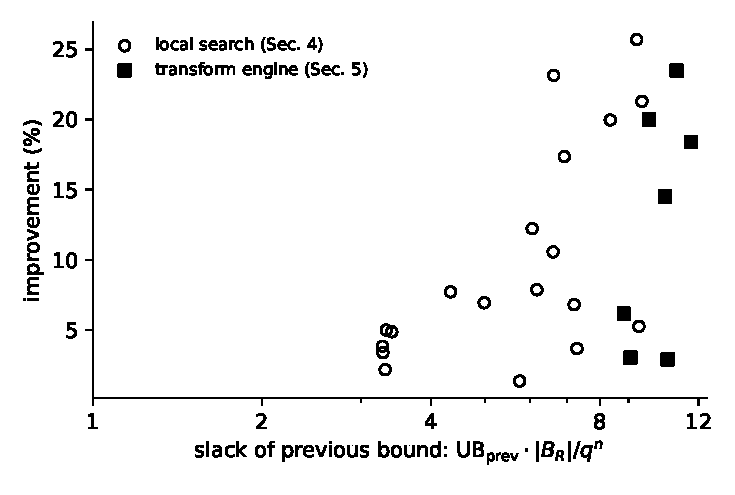
\includegraphics[width=\textwidth]{fig_slack}\\[-1mm]
{\small (a)}
\end{minipage}\hfill
\begin{minipage}[t]{0.48\textwidth}
\centering
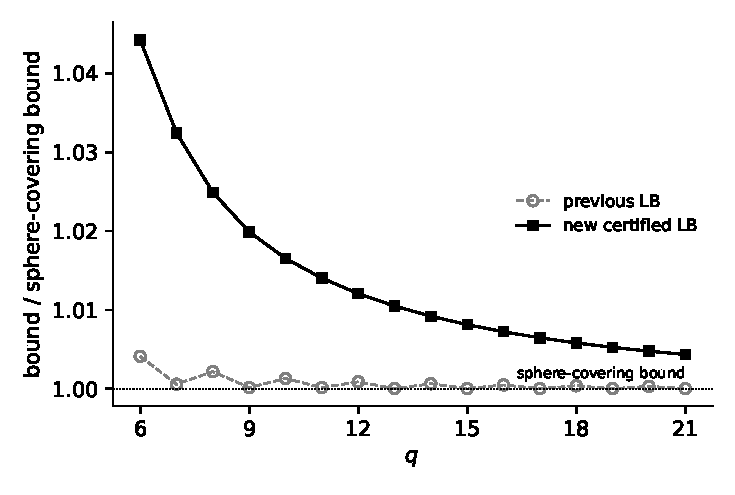
\includegraphics[width=\textwidth]{fig_family82}\\[-1mm]
{\small (b)}
\end{minipage}
\caption{(a) Upper bounds: improvement against the slack of the previous
bound over the sphere-covering bound, for the $25$ cells of
Table~\ref{tab:ub}. Loose bounds inherited from general constructions tend
to fall the furthest (the association is moderate, Spearman
$\rho\approx 0.5$). Squares mark the cells settled by the transform engine of
Section~\ref{sec:gpu}, which operates where $q^n$ puts the cell beyond the
reach of the local search of Section~\ref{sec:method}. (b) Lower bounds:
the family $(n,R)=(8,2)$, $6\le q\le 21$. The previous bounds sit within a
fraction of a percent of the sphere-covering bound, while the certified
semidefinite bound lifts the entire family, by a factor that decreases in
$q$ as predicted by the analysis of the hierarchy
(Section~\ref{sec:lb:limits}).}
\label{fig:summary}
\end{figure}

\begin{remark}\label{rem:keri17}
An audit of the tables of~\cite{Keri} against their own derivation rules
found one internal gap: the tabulated $\Kq{17}{7}{2}\le 252735$ is weaker
than the bound $17\cdot \Kq{17}{6}{2} = 245208$ implied by the tabulated
$\Kq{17}{6}{2}\le 14424$ and the rule $K_q(n{+}1,R)\le q\,K_q(n,R)$. We
record this as an observation; it involves no new construction.
\end{remark}

\section{Upper bounds I: focused local search}\label{sec:method}

\subsection{The search}\label{sec:search}

For fixed $(q,n,R,M)$ we search for a code of size $M$ minimizing the
number of uncovered words. The state is a multiset of $M$ codewords
together with the coverage count $\mathrm{cnt}(w)$ of every $w\in\Zq^n$; a
move changes one coordinate of one codeword.

\begin{lemma}\label{lem:move}
Let $c'$ be obtained from $c$ by setting coordinate $p$ to $v\ne c_p$. Then
the set of words leaving the radius-$R$ ball of $c$ and the set of words
entering the ball of $c'$ are both indexed by the words at distance exactly
$R$ from $c$ in the coordinates other than $p$; consequently a move updates
exactly $2S$ coverage counters with $S=\binom{n-1}{R}(q-1)^R$, the two sets
are disjoint, and distinct counter updates address distinct words.
\end{lemma}

\begin{proof}
Since $d(w,c') = d(w,c) + [\,w_p=c_p\,] - [\,w_p=v\,]$, a word can leave
the ball of $c$ only if $d(w,c)=R$ and $w_p=c_p$, and can enter the ball of
$c'$ only if $d(w,c')=R$ and $w_p=v$, and conversely every word meeting
these conditions leaves (respectively enters); writing such a word as its
restriction to the coordinates $\ne p$ (at distance exactly $R$ from the
restriction of $c$) plus its value at $p$ gives the stated bijections,
disjointness, and injectivity. (All cells considered here have $R<n$;
for $R\ge n$ both sets are empty.)
\end{proof}

The search is a focused local search in the WalkSAT lineage, close in
spirit to the simulated-annealing and tabu searches that produced much of
the original tables~\cite{vanLaarhoven,Ostergard}: select a random
uncovered word $u$;
take as candidates every codeword at distance exactly $R+1$ from $u$ moved
one coordinate towards $u$ (if no codeword is that close, the codewords at
minimum distance from $u$); evaluate all candidates exactly; commit a best
candidate, ties broken uniformly at random; on stagnation, reassign one
codeword to an uncovered word. In parameter studies on $\Kq{6}{6}{3}$,
exact evaluation of all candidates outperformed sampling them, while tabu
tenures and WalkSAT-type noise degraded performance, and simulated
annealing lost to the focused search despite a $33\times$ higher move rate.

Each cell is seeded with a code rebuilt from the construction that produced
the incumbent bound (for $\Kq{6}{10}{4}$, for instance, the direct
sum~\eqref{eq:directsum} of an optimal $\Kq{6}{4}{1}$ code and a
best-known $\Kq{6}{6}{3}$ code, both found by direct search and
verified). Descent proceeds by
remove-and-repair: delete the codeword whose private coverage is smallest
and repair the deficit by search; on success, recurse at $M-1$.

\subsection{Exact reformulations of the evaluation}\label{sec:engineering}

Candidate evaluation dominates the run time (at least $92.9\%$ on all
reference cells), so the search is accelerated by reformulating the
evaluation
exactly rather than by approximating it. The following lemma removes the
per-candidate factor from the dominant term.

\begin{lemma}\label{lem:shared}
With $D(w)=\{j: w_j\neq c_j\}$, a word $w$ leaves the ball of $c$ under the
move at coordinate $p$ if and only if $|D(w)|=R$ and $p\notin D(w)$; it
enters the ball of the moved codeword if and only if $|D(w)|=R+1$,
$p\in D(w)$ and $w_p=v$.
\end{lemma}

\begin{proof}
Immediate from the distance identity in the proof of
Lemma~\ref{lem:move}: $|D(w)|=d(w,c)$, and the move changes the
disagreement set only at coordinate $p$.
\end{proof}

By Lemma~\ref{lem:shared}, with
$T=\#\{w: |D(w)|=R,\ \mathrm{cnt}(w)=1\}$ and
$H_j=\#\{w: |D(w)|=R,\ \mathrm{cnt}(w)=1,\ j\in D(w)\}$, the number of
words newly uncovered by the move at $p$ equals $T-H_p$ for every $p$
simultaneously: a leaving word with $\mathrm{cnt}(w)=1$ has $c$ as its
unique coverer (it lies in the ball of no other codeword) and cannot
simultaneously be re-covered by the moved codeword, since leaving forces
$w_p=c_p\ne v$. One enumeration of the full distance-$R$ sphere of $c$
therefore serves the loss side of all $n(q-1)$ single-coordinate moves of
$c$ at once; the entering (gain) side depends on the written value $v$ and
concerns only words with $\mathrm{cnt}(w)=0$, so maintaining the uncovered
set $U$ explicitly supplies it in $O(n|U|)$ work, an improvement of
two to four orders of magnitude throughout the useful life of a run.
Finally, evaluation reads only whether a counter is $0$ or $1$, so a
two-bit side array $\min(\mathrm{cnt}(w),2)$ serves the read path and
shrinks the read working set into the last-level cache (on $\Kq{8}{9}{4}$,
from $268$\,MB to $33.5$\,MB). Evaluating the widened neighbourhood of all
$n(q-1)$ moves, rather than the $n$ moves towards a focus word, is
profitable on loose cells.

Every reformulation computes the same objective differences as the
reference implementation and therefore follows the same search trajectory
from the same seed; this was verified bit-for-bit over $24$ configurations
spanning $2\le q\le 7$, including the extreme radii $R=0$ and $R=n-1$.
The combined effect is a $2$--$10\times$ speedup at identical trajectories
on the reference cells (largest on the largest cells); the controlled
measurements, together with several
natural optimizations that provably or measurably fail, are reported in
Appendix~\ref{app:impl:cpu}.

\subsection{Structured codes}\label{sec:structure}

Free search over subsets of $\Zq^n$ is the wrong representation for cells
whose optima are algebraic. Two restricted solvers complement it.

\emph{Unions of cosets of a linear code.} When $q$ is a prime power and
$M=c\,q^k$, we search codes of the form $C=\bigcup_{i=1}^{c}(x_i+L)$ with
$L$ a linear $[n,k]_q$ code. Covering then depends only on syndromes: $C$
covers $\Zq^n$ if and only if the $c$ syndromes of the $x_i$ cover the
$q^{n-k}$-element syndrome space under the weight distribution of coset
leaders, reducing a $q^n$-word problem to a $q^{n-k}$-syndrome one. Cells
whose incumbents free search could not even reproduce are settled by this
solver in under a second, e.g.\ $\Kq{8}{8}{4}\le 512=8^3$ and
$\Kq{5}{11}{5}\le 625=5^4$; the descents to the new records $505$ and $602$
then start from verified incumbents.

\emph{Translation quotients.} A second solver searches codes invariant
under $x\mapsto x+\mathbf{1}$ with a free remainder, working in the
quotient of size $q^{n-1}$. On $\Kq{6}{8}{4}$, neither a fully invariant
code (which provably stalls: a single free codeword cannot repair a
deficient orbit) nor a fully free search solves the cell, whereas a mostly
invariant code with a free remainder solves it reliably; at equal
core-seconds on the largest cells the quotient search outperforms free
search by $17\%$.

\subsection{The production configuration}\label{sec:arena}

The production engine merges four independently developed solvers --- the
free search of Section~\ref{sec:engineering}, a low-level SIMD variant,
and the two structured solvers of Section~\ref{sec:structure} --- selected
by a controlled solver competition with held-out evaluation instances and
scoring by independently verified output only; no component won uniformly,
and the merged engine solved at least as many held-out instances as the
best single component. The protocol and its outcome are reported in
Appendix~\ref{app:impl:arena}. An algebraic first phase (the coset solver
over all feasible $k$; seeds from recorded codes and direct sums over all
splits) is followed by a portfolio of independent search chains whose
composition is set by measured thresholds on $q^n$ and the redundancy
$q^n/(M|B_R|)$; a finishing pass re-reads the final code from disk, removes
duplicates, and recomputes coverage by direct ball marking.

All record codes of Table~\ref{tab:ub} marked L (eighteen of the
twenty-five) were produced by this engine on $64$ CPU cores, with per-cell
effort between seconds and a few core-days; the six cells marked T are the
subject of Section~\ref{sec:gpu}.

\section{Upper bounds II: search by exact full-space
transforms}\label{sec:gpu}

Cells with $q^n\gtrsim 10^8$ generally resist the method of
Section~\ref{sec:method}: each chain's working set exceeds the CPU caches
and the per-move sphere walk becomes memory-latency-bound. (The one
exception in Table~\ref{tab:ub} is $\Kq{8}{10}{6}$, whose radius-$6$
balls cover so large a fraction of the space that the uncovered set stays
tiny and the Section~\ref{sec:method} engine remains effective.) Direct ports of
the local search to a GPU do not help --- two were implemented and measured
(Appendix~\ref{app:impl:gpu}), and at best matched one extra CPU socket ---
because the algorithm, not the implementation, is mismatched to the
hardware: its dependent random accesses are mismatched to hardware built
for streaming. The method of this section replaces the pointwise search by
exact whole-space computations.

\subsection{The coverage transforms}

For $S\subseteq\Zq^n$ and $0\le d\le R$ let
$N_d^S(x)=\#\{u\in S: d(x,u)=d\}$. All $R+1$ arrays $N_d^S$ can be
computed simultaneously for \emph{every} $x\in\Zq^n$ by a sequential
transform over the coordinate axes.

\begin{proposition}\label{prop:dct}
Initialize $A_0$ as the indicator of $S$ and $A_1=\dots=A_R=0$. For each
axis $j=1,\dots,n$, update along every one-dimensional fiber
$\{x+t e_j\}_{t\in\mathbb{Z}_q}$:
\[
A_d[a] \;\leftarrow\; A_d[a] + \Bigl(\textstyle\sum_b A_{d-1}[b]\Bigr) -
A_{d-1}[a],
\qquad d=R,\dots,1 .
\]
After all $n$ axes, $A_d = N_d^S$ for every $0\le d\le R$. The total work
is $\Theta\!\left(n R\, q^n\right)$ additions.
\end{proposition}

\begin{proof}
Induction on the number of processed axes: after processing axes
$1,\dots,j$, $A_d(x)$ counts the $u\in S$ that differ from $x$ in exactly
$d$ of the first $j$ coordinates and agree with $x$ elsewhere. The update
adds, for each fiber position $a$, the count of elements at distance $d-1$
in the first $j-1$ axes whose $j$-th coordinate differs from $a$. The
descending order $d=R,\dots,1$ is essential to the in-place formulation:
the update for $A_d$ must read the values of $A_{d-1}$ from the
\emph{previous} axis, which the descending order preserves ($A_{d-1}$ is
overwritten only after every $A_d$ that reads it); $A_0$ is never
modified, correctly, as the indicator of $S$ restricted to agreement on
processed axes. Two implementation conditions are part of the statement:
within each fiber the grade loop $d=R,\dots,1$ is the \emph{outer} loop
(so no position of the fiber sees a partially updated neighbour), and the
fiber sum $\sum_b A_{d-1}[b]$ is formed once per fiber and grade before
any write; the $\Theta(nRq^n)$ count assumes both.
\end{proof}

The transform is an instance of the classical fast product-domain
technique going back to Yates~\cite{Yates}, applied to the
distance-graded filtration and truncated at grade $R$; what matters here
is not novelty but the pairing with exact search primitives, as follows.

The update is branchless and uniform over $q^{n-1}$ independent fibers ---
a bandwidth-bound workload on which a GPU operates at its design point. On
the node used here (specified in Appendix~\ref{app:impl}), the full
transform takes $63$\,ms at
$q^n=7^{10}$ and $143$\,ms at $8^{10}$ with $32$-bit counters (memory
footprint $4(R+1)+2$ bytes per word of the space).

Two instances of Proposition~\ref{prop:dct} give global exact information
that pointwise local search cannot afford. With $S$ the set of uncovered
words, $g(x)=\sum_{d\le R}N_d^S(x)$ is the exact number of words newly
covered by a codeword placed at $x$, for every candidate position $x$
simultaneously; with $S$ the set of words covered exactly once,
$\ell(c)=\sum_{d\le R}N_d^S(c)$ is the exact number of words that would be
uncovered by deleting $c$, for every codeword $c$.

\subsection{The search}

The engine is a large-neighbourhood search over these primitives: starting
from a seed code (a direct-sum construction or a recorded code), delete a
set of codewords chosen by low $\ell$-value (mixed with randomized
removals), then rebuild by repeatedly placing a codeword at the maximizer
of the current gain map $g$, recomputing or locally correcting $g$ after
each placement; a completed cover at size $M$ triggers a descent attempt at
$M-1$ by the same remove-and-rebuild step. Each placement is thus globally
optimal with respect to exact coverage information, in contrast to the
single-coordinate moves of Section~\ref{sec:method}; the engine performs
far fewer moves of far higher quality. The greedy rebuild is also an
effective constructor from an empty code: on $\Kq{8}{10}{4}$
($q^n=1.07\cdot 10^9$) it builds a full cover of size $14946$ in three
minutes, a task on which the CPU engine failed outright.

Five of the bounds of Table~\ref{tab:ub} were produced by this engine on
cells with $2.8\cdot 10^8\le q^n\le 3.5\cdot 10^9$, within hours and
including reductions of $20.0\%$ ($\Kq{7}{10}{5}$), $23.5\%$
($\Kq{8}{10}{5}$) and $14.5\%$ ($\Kq{9}{10}{5}$); all were verified by the
independent protocol of Section~\ref{sec:verify}. With every array
resident in GPU memory the engine reaches $q^n\approx 3.5\cdot 10^9$;
Section~\ref{sec:gpu:hc} removes that ceiling.

\subsection{Reaching $q^n=10^{10}$}\label{sec:gpu:hc}

With every array resident in GPU memory, the largest searchable cells have
$q^n\approx 3.5\cdot 10^9$ --- which is precisely where K\'eri's tables
keep several of their loosest entries: $\Kq{10}{10}{5}$ ($q^n=10^{10}$,
upper bound $7106$ against a sphere-covering bound of $612$) and its
neighbours sit one order of magnitude beyond that ceiling. The ceiling is
removed by placing the streaming layer arrays of
Proposition~\ref{prop:dct} in the node's much larger CPU-attached memory,
which the GPU addresses coherently, while the randomly-accessed
multiplicity array stays in GPU memory; a transform then costs roughly
$24$ times more, but the whole of K\'eri's $q\le 10$ tables becomes
feasible on one node. The measured costs, and the memory-placement
details required to reproduce them, are collected in
Appendix~\ref{app:impl:gpu}.

This configuration produced the record on the largest cell attempted: on
$\Kq{10}{10}{5}$, exact greedy construction followed
by the large-neighbourhood descent reached $\Kq{10}{10}{5}\le 5799$ against
the previous bound $7106$ (a direct sum), a reduction of $18.4\%$, within
six hours of a single node --- to our knowledge the first covering-code
bound established by exhaustive-evaluation search over a space of $10^{10}$
words. The code was verified by the full protocol of
Section~\ref{sec:verify}.

\subsection{Limits: private-uniform incumbents}\label{sec:gpu:rigid}

The engine's failures also delimit the method. The
K\'eri upper bound $\Kq{8}{10}{4}\le 11776$ is a direct sum
$23\times 512$ of a $\Kq{8}{4}{2}$-code and a $\Kq{8}{6}{2}$-code. Product
structure makes the incumbent \emph{private-uniform}: every codeword
privately covers ${\approx}9800$ words (measured on the incumbent, which
is reconstructible from its stated factors), roughly seven times the
${\approx}1350$ a random code of equal size would privately cover in
expectation, so the deletion of any $k$ codewords instantly
owes ${\sim}9800k$ words that a same-size rebuild must repay exactly. In a
dedicated eight-hour attack with ruins of up to $512$ codewords beyond the
target deficit, removal of even a \emph{single} codeword below the
incumbent could not be repaired: the best residual over three attempts
with budgets escalating to $2.6$ hours was $77229$ uncovered words, and
larger deficits fared worse. The same holds for
$\Kq{9}{10}{4}=27\times 729$. We conclude that word-level
ruin-and-recreate, however exact its evaluations, cannot dismantle a
product construction whose loss landscape is flat and high everywhere;
progress on
these cells requires moves in the factor spaces (replacing the
$\Kq{8}{4}{2}$ factor of size $23$ by one of size $22$, if it exists,
would give $\Kq{8}{10}{4}\le 11264$ outright) or seeds with genuine slack. (The factor-space move was attempted: six independent
four-hour searches for a $\Kq{8}{4}{2}$-code of size $22$ --- the open
K\'eri gap is $22$--$23$ --- all stalled at exactly $36$ uncovered words
of the $4096$; the cell remains open.)
By contrast, the loose high-redundancy incumbents of the same tables
(ratio to the sphere-covering bound above ${\approx}8$) fall to the exact
greedy constructor alone; the boundary between the two regimes is the
practical content of this subsection.

\begin{remark}
Nothing in the engine below the transform is specific to covering codes:
the search interacts with the problem only through the gain and loss
fields of Proposition~\ref{prop:dct} and a table describing one solution
element's support set. Any covering-type problem over a product space
$\prod_j \mathbb{Z}_{m_j}$ whose neighbourhood admits a separable per-axis
transform fits the same machinery; as an existence proof, an
implementation for dominating sets of torus grids under king-move balls
runs through the unchanged search core and was validated exhaustively
against brute force on small instances. A systematic treatment is
deferred to follow-up work.
\end{remark}

\section{Lower bounds: exact certificates from a multiprecision
SDP pipeline}\label{sec:lb}

\subsection{The relaxation and its exact reconstruction}

Gijswijt and Polak~\cite{GijswijtPolak} bound $K_q(n,R)^3$ from below by a
semidefinite program over variables indexed by orbits of triples of words
under $\mathrm{Aut}(q,n)=S_q\wr S_n$, with positive-semidefiniteness
constraints from the block-diagonalization of the Terwilliger algebra of
the Hamming scheme, linear constraints from sphere-covering inequalities,
and matrix-cut constraints (their Proposition~4.17; the full
symmetry-reduced bound is their Theorem~4.18). For $q\ge 3$ the size of
the reduced program depends only on $n$ --- at $n=11$ it has $339$
variables and $126$ blocks of order at most $13$ --- while $q$ enters only
through the coefficients; published computations stop at $q\le 5$.

We reimplemented the reduced program with the entire model generation in
exact integer arithmetic and validated the implementation four ways:
(a) a self-test that substitutes explicit verified covering codes into the
model and checks every constraint in exact rational arithmetic, with
objective exactly $|C|^3$; (b) a coefficient-level comparison against the
authors' published code, matching every generated coefficient over six
$(q,n,R)$ cells spanning $3\le q\le 7$; (c) reproduction of the published
values: of $49$ published table values recomputed, $44$ agree to display
precision, and $18$ of the $22$ published improved lower bounds attempted
are reproduced exactly at the integer level --- the four integer-level
misses ($\Kq{4}{7}{1}$ by $1$, $\Kq{5}{7}{1}$ by $7$, $\Kq{5}{8}{1}$ and
$\Kq{5}{8}{2}$) all lie where double precision is known to fail, this
validation stage predating the multiprecision pipeline of
Section~\ref{sec:lb:numerics}, which subsequently reproduced the hardest
of them, $\Kq{5}{8}{2}\ge 861$, exactly; every recomputed value is itself
a certified lower bound on the same optimum, so no such discrepancy can
inflate a bound; (d) the invariant that no
certified lower bound may exceed a known upper bound, checked against all
$1145$ table cells and never violated.

\subsection{Certification}\label{sec:lb:cert}

Numerical solutions are used only as suggestions. By weak duality, any
feasible point of the dual program --- multipliers $y_k\ge 0$ for the
linear constraints and positive semidefinite matrices $Y_b$ for the blocks
--- certifies the bound it attains. Each numerical dual solution is rounded
to rationals over a dyadic denominator, each $Y_b$ is displaced strictly
into the semidefinite cone, and, should any dual inequality fail in exact
arithmetic, the entire dual is scaled by a dyadic factor $\theta\le 1$,
which restores feasibility at proportional cost in the bound.

The resulting certificate is validated by a standalone checker (Python
standard library only) that re-derives the entire
program from $(q,n,R)$ in exact integer arithmetic, verifies $y_k\ge 0$,
verifies each $Y_b\succeq 0$ by exact $LDL^{\mathsf T}$ factorization over
the rationals, verifies every dual inequality in integer arithmetic, and
extracts the integer bound by exact cube-root comparison. The checker also
verifies that the covering inequality named in the certificate is itself
valid, so that an unsound constraint cannot be smuggled in. The precise
statement of the certified program, and of what a certificate proves, is
given in Appendix~\ref{app:sdp}. The trusted
base is therefore twofold, and we state it honestly: the checker's
validation logic, and the transcription of the reduced program
of~\cite{GijswijtPolak} into the model generator, which the checker shares
with the solving pipeline; a transcription error invalid for every
covering code would not be caught by the certificate, which is why the
transcription is validated separately by the four tests of the previous
subsection. No floating-point computation enters either component.

\subsection{Numerical solution}\label{sec:lb:numerics}

Two numerical issues govern whether a good dual point can be found at all.
First, conditioning: the optimum $|C|^3$ may exceed $10^{13}$ while every
constraint constant is $O(1)$, and the objective coefficients span ten
orders of magnitude. All computations therefore use a geometric-mean
equilibration --- normalize the objective by the cube of the
sphere-covering bound and give each variable the magnitude profile of the
square root of its objective contribution --- applied entirely in powers of
two, so that the map back to the unscaled dual is exact. On $\Kq{6}{8}{3}$
(in the double-precision stage) equilibration raises the certified bound
from $K\ge 183$ to $K\ge 240$; since the cube root of the relaxation
optimum is ${\approx}239.52$, the integer bound $240$ is the best the
relaxation can give.

Second, precision. In IEEE double precision, interior-point solvers fail
beyond optima of roughly $1.5\cdot 10^9$ (cube root ${\approx}1150$), which
excludes most of the cells with the largest head-room. All $58$
certificates of Table~\ref{tab:lb} therefore come from multiprecision
solves with SDPA-GMP~\cite{sdpagmp} at $200$- or $250$-bit precision,
compiled natively for the target architecture. (The ancillary collection
also retains earlier certificates produced by a double-precision
interior-point stage; they pass the same exact checker but are generally
weaker, and none of them underlies Table~\ref{tab:lb}.) The problem
files are written with exact dyadic coefficients, the multiprecision dual
is parsed into exact rationals, and rounding is performed \emph{in the
equilibrated coordinates} over denominator $2^{128}$, with the
displacement into the semidefinite cone tied to the rounding grain. With
these choices, $52$ of the $58$ certificates underlying Table~\ref{tab:lb}
attain $\theta=1$, and the remaining six have
$\theta\ge 1-2.3\cdot 10^{-4}$, the loss never affecting the integer
bound: essentially nothing of the numerically obtained value is lost in
certification. As an end-to-end anchor, the pipeline reproduces the
published $512$-bit value $\Kq{5}{8}{2}\ge 861$ of~\cite{GijswijtPolak}
exactly.

\subsection{Extent and limits of the method}\label{sec:lb:limits}

The improvements land where the analysis of the hierarchy predicts. At this
level the semidefinite bound exceeds the sphere-covering bound by a factor
that decreases in $q$ (on the scale of $K$ itself, i.e.\ after the cube
root; for $(n,R)=(8,4)$: $1.44$ at $q=4$ down to $1.16$
at $q=7$), so it overtakes the tabulated bounds precisely where those are
close to sphere-covering: the improved cells all carry keys \texttt{y},
\texttt{x}, \texttt{s} or \texttt{a}, and complete families such as
$(n,R)=(8,2)$, $6\le q\le 21$, fall at once
(Figure~\ref{fig:summary}(b)).

The pipeline also gives evidence of limits. On the twelve cells
$\Kq{q}{7}{3}$, $15\le q\le 18$, $\Kq{q}{8}{3}$, $q\in\{14,15,16,20\}$,
and $\Kq{q}{8}{4}$, $18\le q\le 21$, the solver converges to its working
precision at a value strictly \emph{below} the tabulated bound, and the
rounded dual certifies that value up to a factor
$\theta\ge 1-2.4\cdot 10^{-4}$ (with $\theta=1$ on two of them). We are
explicit about the logical status of this statement: a dual certificate
proves only a \emph{lower} bound on the optimum of the relaxation, so the
impossibility of improvement on these cells is attested by the solver's
convergence, not by exact arithmetic. The distinction matters: the
ancillary collection also contains duals from failed solves whose
certified values fall even below the sphere-covering bound (e.g.\
$\Kq{9}{6}{2}$), so a value below the tabulated bound is meaningful only
together with the solver's terminal status. On all twelve cells above,
SDPA-GMP terminated in phase \texttt{pdOPT} --- primal and dual feasible
with relative gap below the solver tolerance at $200$-bit working
precision. An exact impossibility proof would
require a rational \emph{primal} feasible point with value below the cube
of the tabulated bound, which we have not pursued. In the extreme case
$R=1$ the hierarchy tracks the sphere-covering bound closely at $q\ge 6$:
for $\Kq{6}{7}{1}$ the certified value equals the sphere-covering bound
$7776=6^7/36$ exactly, and for $\Kq{6}{8}{1}$ it exceeds the
sphere-covering bound by only $1.5\%$ while remaining below the tabulated
$41991$. Against the strong combinatorial bounds of Haas, Halupczok and
Schlage-Puchta~\cite{HHSP2009} (key \texttt{m}, $11$--$67\%$ above the
sphere-covering bound on the cells we attempted) the relaxation is weaker
throughout the range considered.
We also note that the fractional covering \emph{linear} program cannot
improve any cell: every word of $\Zq^n$ lies in exactly $|B_R|$ balls, so
summing all covering constraints shows the LP optimum is at least
$q^n/|B_R|$, while the uniform solution attains it; the LP optimum is thus
exactly $q^n/|B_R|$, whose ceiling is the sphere-covering bound.

\section{Verification}\label{sec:verify}

Every bound in this paper was verified independently of the software that
produced it.

\emph{Upper bounds.} Every claimed code, re-read from its published file,
was checked by four methods, two of which share no code with the other
two: (i) ball marking over a $q^n$ bitmap; (ii) meet-in-the-middle bitset
covering over a coordinate split; (iii) a min-distance scan over all $q^n$
words, which also reports the exact covering radius; (iv) $R$-fold
neighbourhood dilation of the code's indicator array, which computes no
distances at all. A fifth dilation check, written independently of the
verifiers and included in the repository's build script, re-confirmed all
$25$ codes from the published files immediately before
this version was prepared; the largest check covers
$10^{10}$ words. The distinct-codeword count of every file
is checked against the claimed $M$. (Re-verifying the largest records is
itself a computation: the $\Kq{9}{10}{5}$ dilation needs a few GB of
memory and minutes, the $\Kq{10}{10}{5}$ check tens of GB or the
meet-in-the-middle method; the ancillary README states the resource needs
per record.)

\emph{Lower bounds.} Every certificate was re-validated by the exact
checker of Section~\ref{sec:lb:cert} immediately before this version was
prepared ($196$ certificates: $58$ improving on the tabulated lower
bound, $28$ whose certified integer bound equals the tabulated value, the
remainder falling short of the tabulated value or concerning cells
without one; none exceeds a known upper bound).

The ancillary files contain all codes (one codeword per line, digits
\texttt{0}--\texttt{9} then \texttt{a}--\texttt{z} for $q>10$), all $58$
record certificates, and both standalone verifiers
(\texttt{verify\_cov.py} and \texttt{certify.py}), each dependency-free.

\section{Concluding remarks}

The upper-bound experiments show a tendency, not a law: across the
improved cells (whose previous bounds have slack $3.3$--$11.6\times$ over
the sphere-covering bound) larger slack broadly permits larger
improvements, up to $23\%$, while bounds set by dedicated search in the
2000s fall by $2$--$12\%$; the association in
Figure~\ref{fig:summary}(a) is moderate (Spearman
$\rho\approx 0.5$), and individual loose cells can still resist. The transform-based engine of Section~\ref{sec:gpu}
extends the reachable range to $q^n=10^{10}$ and none of the
large-cell descents has yet stalled, so further improvements are expected
from computation alone. On the lower-bound side, the multiprecision
pipeline has exhausted neither the alphabet range nor the hierarchy: the
van Wee-type strengthenings of the linear constraints, used
in~\cite{GijswijtPolak} for $q=2$ only, and the conditional use of known
upper bounds are both untried at $q\ge 6$, while the closed-cell evidence
of Section~\ref{sec:lb:limits} delimits what the present level can
achieve.

Since the tables of~\cite{Keri} have had no maintainer since 2011, a
merged machine-readable bounds table (K\'eri 2011, the post-2011
literature, and the present improvements) is published alongside the code.

\subsection*{Data availability}
The codes, the certificates, both verifiers, and a README are ancillary
files of the arXiv version of this paper. The full search, certification,
and verification source code, together with the merged bounds table, is
available at \url{https://github.com/Mapika/coldcase}.

\subsection*{Contributions and acknowledgments}
The author conceived the research programme and directed it throughout;
its decisive turns were the author's: the initiating idea of attacking record
tables frozen since the 2000s with modern large-scale search; the decision
to pursue certified lower bounds alongside constructive upper bounds; the
insistence, when direct GPU ports of the local search failed, that the
problem be reformulated in the dense, branchless form natural to the
hardware, from which the transform engine of Section~\ref{sec:gpu}
resulted; the competitive solver-selection methodology of
Section~\ref{sec:arena}; the sustained selection of which cells and
problem transformations to pursue; and the computational resources. The
software, the mathematical elaboration, the computations, and the drafting
of this manuscript were carried out, under the author's direction, by the
AI system Claude (Anthropic), whose contribution the author gratefully
acknowledges as substantial and essential. Every bound was verified by the
protocol of Section~\ref{sec:verify} independently of the software that
produced it.

\bibliographystyle{amsplain}
\bibliography{refs}

\appendix

\section{Implementation notes and controlled measurements}\label{app:impl}

This appendix collects the engineering measurements supporting the claims
of Sections~\ref{sec:method} and~\ref{sec:gpu}. All comparative figures
are process CPU time or paired same-window measurements on the same node
(an NVIDIA GH200: $64$ ARM cores, $480$\,GB LPDDR, H100-class GPU with
$96$\,GB HBM); wall-clock comparisons across different loads are never
used.

\subsection{The evaluator of Section~\textup{\ref{sec:engineering}}}
\label{app:impl:cpu}

Profiling shows candidate evaluation accounting for $92.9\%$, $98.5\%$
and $99.6\%$ of run time on three reference cells of increasing size
($\Kq{6}{6}{3}$ at $M=41$, $\Kq{6}{8}{4}$ at $M=169$, $\Kq{8}{9}{4}$ at
$M=2944$), with the cost of one evaluated sphere pattern rising from
$1.9$\,ns to $7.4$\,ns as the counter array grows from cache-resident
($93$\,kB) to DRAM-resident ($268$\,MB).
Table~\ref{tab:engfixed} isolates the implementation effect at fixed
search trajectory; Table~\ref{tab:engttt} measures end-to-end time to a
fixed quality target.

\begin{table}[ht]
\centering
\begin{tabular}{lccc}
\toprule
variant & $\Kq{6}{6}{3}$ & $\Kq{6}{8}{4}$ & $\Kq{8}{9}{4}$ \\
        & 20\,000 it & 600 it & 50 it \\
\midrule
reference implementation      & $1.00\times$ & $1.00\times$ & $1.00\times$ \\
peeled walk, hoisted offsets  & $1.35\times$ & $1.29\times$ & $1.13\times$ \\
\quad + 8-bit state array     & $1.28\times$ & $1.65\times$ & $1.65\times$ \\
\quad + 2-bit state array     & $0.82\times$ & $1.34\times$ & $2.44\times$ \\
shared sphere, 8-bit state    & $1.32\times$ & $1.95\times$ & $1.95\times$ \\
\quad + uncovered-word list   & $2.21\times$ & $5.57\times$ & $6.06\times$ \\
\quad with 2-bit state        & $2.14\times$ & $\mathbf{6.32\times}$ & $\mathbf{9.86\times}$ \\
\bottomrule
\end{tabular}
\caption{Speedup in CPU time at a fixed iteration budget, median of $9$
runs ($6$ on the largest cell). Every row performs the identical search:
final uncovered counts agree exactly, seed by seed, across rows.
Interquartile ranges are $0.9\%$, $2.2\%$ and $5.6\%$ of the median.}
\label{tab:engfixed}
\end{table}

\begin{table}[ht]
\centering
\begin{tabular}{lcccc}
\toprule
cell & $M$ & target & identical search & wide neighbourhood \\
\midrule
$\Kq{6}{6}{3}$ & 41   & $|U|\le 30$      & $2.03\times$ $[1.99,2.13]$ & $0.28\times$ \\
$\Kq{6}{8}{4}$ & 169  & $|U|\le 20$      & $6.12\times$ $[6.06,6.62]$ & $8.03\times$ $[5.75,11.02]$ \\
$\Kq{8}{9}{4}$ & 2944 & $|U|\le 10\,800$ & $8.07\times$ $[6.19,10.72]$ & $11.04\times$ $[8.06,12.17]$ \\
\bottomrule
\end{tabular}
\caption{Median per-seed speedup in CPU time to target over $20$ seeds,
with percentile-bootstrap $95\%$ confidence intervals. In the fourth
column the optimized solver reached the target at the same iteration as the
reference on all seeds, so the ratio is a pure implementation speedup; the
fifth column also widens the candidate neighbourhood, which changes the
search (fewer iterations to target on the two loose cells, a $3.6\times$
loss on the tight one).}
\label{tab:engttt}
\end{table}

Several natural optimizations fail for structural reasons, which we
record. Caching move evaluations between iterations requires evaluation
spheres to be disjoint, i.e.\ $d(c,c')>2R+2$; since $2R+2\ge n$ on every
cell of interest, every commit invalidates every cache entry. Maintaining
the singly-covered analogue of $U$ pays only if
$n|U_1|<\binom{n}{R}(q-1)^R$, which fails by one to two orders of magnitude
--- uncovered words are rare by construction, singly covered words are not.
Translation symmetry reduction (fixing one codeword at $0^n$) yields no
measurable benefit, since a local search does not revisit states. A
deterministic focus rule (always the longest-uncovered word) is severely
harmful, destroying the randomization that lets focused search leave
plateaus. Restart schedules help only where the run-time distribution to
the target is heavier than exponential, which occurs on tight cells
(observed speedup $4.2\times$, $p=0.002$, on $\Kq{6}{6}{3}$ at a hard
target) and not on the loose cells this paper improves (coefficient of
variation $0.20$--$0.47$; $p=1.0$).

\subsection{The solver competition of Section~\textup{\ref{sec:arena}}}
\label{app:impl:arena}

Four independently developed implementations --- the engineered free
search, a low-level SIMD variant, the structured solvers, and a portfolio
scheduler --- were compared under a fixed protocol: identical interface
and resource limits, public development instances, held-out evaluation
instances, $15$ seeds per instance, and scoring by independently verified
output only (a full verified cover scores $1000$; a partial cover scores
the negated uncovered fraction; invalid output scores below any valid
partial). No component won uniformly: the structured solvers dominated the
held-out evaluation, the engineered evaluator was fastest on large cells,
the SIMD variant on cache-resident cells, and many single-threaded chains
beat multi-threaded ones except on the largest cells. Under the frozen
protocol the merged engine of Section~\ref{sec:arena} solved at least as
many held-out instances as the best single component ($14/20$ against
$12/20$).

\subsection{GPU measurements for Section~\textup{\ref{sec:gpu}}}
\label{app:impl:gpu}

\emph{Direct ports that fail.} A formulation of candidate evaluation as
integer matrix products (to engage tensor cores) is starved by its
contracted dimension of only $nq\approx 50$ and never approached CPU
throughput. A port running $256$ independent chains in one persistent
kernel reaches $0.09\times$, $0.10\times$ and $1.24\times$ the throughput
of the full $64$-core socket on cells with $q^n=4.7\cdot 10^4$,
$1.7\cdot 10^6$ and $1.3\cdot 10^8$ respectively --- at best one extra
socket, obtained only where the CPU is already at its worst. These
measurements motivated the change of algorithm in Section~\ref{sec:gpu}.

\emph{Memory placement for $q^n>3.5\cdot 10^9$
(Section~\textup{\ref{sec:gpu:hc}}).} The node pairs the GPU ($96$\,GB
HBM) with $480$\,GB of CPU-attached LPDDR memory behind a cache-coherent
interconnect: a GPU thread can dereference any CPU pointer, with native
atomics, at interconnect rather than PCIe cost. Each array is placed
independently: the layer arrays, touched only by the streaming axis
passes, go to LPDDR; the multiplicity array $\mathrm{cnt}$, dominated by
random-access ball walks, stays in HBM (for $\Kq{10}{10}{5}$: $240$\,GB
LPDDR, $21$\,GB HBM). One finding matters for reproduction: the placement
must be \emph{pinned}. Allocation through the unified-memory allocator is
a factor ${\sim}30$ slower than plain \texttt{malloc} accessed through the
coherent page tables, and plain \texttt{malloc} is not stable either,
because the default kernel policy migrates GPU-hot pages into HBM until it
overflows and thrashes; binding the allocations to the CPU NUMA node
(\texttt{mbind}) makes the placement deterministic. Outputs were verified
bit-identical across all placements. Table~\ref{tab:hc} gives the measured
cost of one full coverage transform (the unit of work of every search
round) across placements.

\begin{table}[ht]
\centering
\begin{tabular}{lrrrr}
\toprule
cell & $q^n$ & arrays & placement & transform \\
\midrule
$\Kq{8}{10}{4}$ & $1.1\cdot 10^9$ & $24$\,GB & HBM & $0.143$\,s \\
$\Kq{8}{10}{4}$ & $1.1\cdot 10^9$ & $24$\,GB & LPDDR (pinned) & $3.4$\,s \\
$\Kq{8}{10}{4}$ & $1.1\cdot 10^9$ & $24$\,GB & LPDDR (managed) & $8.7$\,s \\
$\Kq{9}{10}{5}$ & $3.5\cdot 10^9$ & $91$\,GB & LPDDR (pinned) & $22$--$26$\,s \\
$\Kq{10}{10}{5}$ & $10^{10}$ & $260$\,GB & LPDDR (pinned) & $73$--$110$\,s \\
\bottomrule
\end{tabular}
\caption{One exact coverage transform by array placement (idle node; LPDDR
rows keep the multiplicity array in HBM). The LPDDR penalty of
$\sim\!24\times$ buys an order of magnitude of problem size, and the
ball-walk primitives --- the other half of each search round --- remain
HBM-resident, so the large-neighbourhood search still executes at a viable
rate.}
\label{tab:hc}
\end{table}

\emph{Kernel-level optimizations of the transform engine.} Ball walks are
driven by a precomputed table of packed coordinate-shift patterns, so each
visited word costs one table load and at most $R$ shared-memory adds, with
no division or modulo in the hot loop. Splitting each walk over up to
$8192$ thread blocks (the original engine used one) makes single-word
updates --- the innermost operation of the exact lazy-greedy rebuild ---
$30\times$ faster on $\Kq{8}{9}{4}$ ($0.80\to 0.027$\,ms) and $37\times$
faster on $\Kq{8}{10}{4}$ ($1.34\to 0.036$\,ms), batched candidate
evaluations $3.7$--$4.3\times$ faster, and a complete exact-greedy cover
construction on $\Kq{8}{9}{4}$ $1.4\times$ faster end to end at identical
cover size; the change is pure scheduling. An alternative
register-resident table format performs within measurement noise of the
packed-byte format, and the engine retains both. One transplanted idea is
recorded as a negative result: tagging each word's last coverer during the
mark pass, so that per-codeword losses fall out of one linear scan,
replaces one transform but loses to it ($28$ vs.\ $17$\,ms on
$\Kq{8}{9}{4}$, $669$ vs.\ $145$\,ms on $\Kq{8}{10}{4}$), because the mark
pass re-walks every codeword's ball ($M\cdot|B_R|$ atomic operations)
where the transform streams $O(nRq^n)$ words; it wins only where
$M\cdot|B_R|\ll nRq^n$, a regime the record cells do not enter.

\section{The certified program and the meaning of a
certificate}\label{app:sdp}

This appendix states precisely what a certificate of Table~\ref{tab:lb}
proves, so that the certificates have paper-level semantics independent of
any implementation. The reduced program of~\cite[Theorem~4.18]{GijswijtPolak}
(non-binary case, $q\ge 3$) is a linear--semidefinite minimization in
variables $x\in\mathbb{R}^N$ indexed by the orbits of triples of words
under $\mathrm{Aut}(q,n)=S_q\wr S_n$:
\begin{equation}\label{eq:sdp}
\begin{aligned}
\min\; c^{\mathsf T}x
\quad\text{s.t.}\quad
& x\ge 0,\qquad
\langle l_k,x\rangle + l_k^0 \ge 0 \quad (k=1,\dots,m),\\
& C_b + \textstyle\sum_{v=1}^{N} x_v A_b^v \succeq 0 \quad (b=1,\dots,B),
\end{aligned}
\end{equation}
where the data $c$, $(l_k,l_k^0)$, $(C_b,A_b^v)$ are explicit rationals
determined by $(q,n,R)$: the objective and the linear constraints encode
sphere-covering inequalities and the matrix-cut inequalities
of~\cite[Proposition~4.17]{GijswijtPolak}, and the semidefinite blocks
arise from the block-diagonalization of the Terwilliger algebra of the
nonbinary Hamming scheme~\cite[\S 3]{GijswijtPolak}. The property that
gives the program its meaning is
\cite[Theorem~4.18]{GijswijtPolak}: \emph{every} code
$C\subseteq\Zq^n$ of covering radius at most $R$ induces a feasible point
$x_C$ of~\eqref{eq:sdp} with $c^{\mathsf T}x_C=|C|^3$. Consequently
$K_q(n,R)^3\ge\mathrm{OPT}$, the optimum of~\eqref{eq:sdp}.

A certificate for the pair $(q,n,R)$ is a vector $y\in\mathbb{Q}^m_{\ge 0}$
together with rational symmetric positive semidefinite matrices
$Y_1,\dots,Y_B$ (all stored over one common denominator). Define
\[
d_v \;=\; \sum_k y_k\, l_k[v] \;+\; \sum_b \langle Y_b, A_b^v\rangle
\quad (v=1,\dots,N),
\qquad
d_0 \;=\; \sum_k y_k\, l_k^0 \;+\; \sum_b \langle Y_b, C_b\rangle .
\]

\begin{lemma}\label{lem:cert}
If $d_v\le c_v$ for every $v$, then every feasible point $x$
of~\eqref{eq:sdp} satisfies $c^{\mathsf T}x\ge -d_0$; hence
$K_q(n,R)\ge\bigl\lceil(-d_0)^{1/3}\bigr\rceil$.
\end{lemma}

\begin{proof}
For feasible $x$,
\[
c^{\mathsf T}x + d_0
= \sum_v (c_v-d_v)\,x_v
+ \sum_k y_k\bigl(\langle l_k,x\rangle + l_k^0\bigr)
+ \sum_b \Bigl\langle Y_b,\; C_b+\sum_v x_v A_b^v\Bigr\rangle
\;\ge\; 0,
\]
since each summand is a product of nonnegative quantities ($x\ge 0$ and
$c_v-d_v\ge 0$; $y_k\ge 0$ and the linear constraint value $\ge 0$; and
the inner product of two positive semidefinite matrices is nonnegative).
The bound on $K_q(n,R)$ follows from
$K_q(n,R)^3\ge\mathrm{OPT}\ge -d_0$.
\end{proof}

If the rounding of a numerical dual leaves some $d_v>c_v$, the entire
certificate is scaled by the largest dyadic $\theta\le 1$ with
$\theta d_v\le c_v$ for all $v$, which preserves feasibility of the scaled
certificate and yields the bound $-\theta d_0$. The checker validates
exactly the hypotheses of Lemma~\ref{lem:cert} --- nonnegativity of $y$,
positive semidefiniteness of each $Y_b$ by exact $LDL^{\mathsf T}$
factorization over $\mathbb{Q}$, and the $N$ inequalities $d_v\le c_v$ in
integer arithmetic --- and re-derives the data
$c,(l_k,l_k^0),(C_b,A_b^v)$ from $(q,n,R)$ alone; the transcription of
that data from~\cite{GijswijtPolak} is the assumed part of the trusted
base, validated as described in Section~\ref{sec:lb}.

\section{The code proving $\Kq{6}{8}{4}\le 166$}\label{app:code}
The largest relative single improvement among the converged cells
($216\to 166$) is printed for self-containedness; each row lists codewords
of $\mathbb{Z}_6^8$, and the machine-readable version is the ancillary file
\texttt{K6\_8\_4\_M166.txt}.

{\scriptsize
% AUTO-GENERATED by scripts/paper_tables.py
\begin{verbatim}
01430421  12541532  23052043  30103154
45214205  50325310  03405225  14510330
25021441  30132552  41243003  52354114
03134001  14245112  25350223  30401334
51512445  52010550  02442243  13553304
24004415  35115520  40220031  51331142
02303231  13414342  24525453  35030504
40141015  51252120  05143544  10254055
21305100  32410211  43521322  54032433
04301535  13432040  20543151  31054202
42105313  53210434  04043240  15154351
20205402  31310513  42421024  53532135
05111133  10222244  21333355  32444400
43555511  54000022  01045452  12150503
23201014  34312125  45423230  50534341
00544125  11055230  22100341  33211452
44322503  55433014  02231500  13342011
24453122  35504233  40015344  51120455
05223315  10334420  21445531  32550042
43001153  54112204  03411050  14542101
25033212  30144323  41255434  52300445
04450305  15501410  20012521  31123032
42234143  53345254  00052413  11103524
22214035  33324140  44430251  55541302
02115012  13220123  24331234  35442345
40553450  51004501  01024314  12135425
23240530  34351041  45402152  50513203
05352332  10413443  21514554  52025505
43130110  54241221  04205542  15315053
20420104  31531215  42042320  53153431
01213111  12324222  23435333  34540444
45051555  42131403  00300252  11411303
22522414  33033525  44104030  55255141
05535024  10040135  21151240  32202351
44313402  54424513  01500043  12051134
23122205  34233310  45344421  50455532
03314404  10402515  25530020  31021031
41132242  52243353  12005001  03402520
31455113  23344502  55203541  32515205
30325000  02023150  14021545  54142054
34124521  03523252  45250342  00522424
44553234  53044110
\end{verbatim}

}

\end{document}
